\documentclass[11pt,a4paper,openright,twoside]{article}
\usepackage[english]{babel}
\usepackage{newlfont}
\usepackage{color}
\textwidth=450pt\oddsidemargin=0pt
\usepackage{graphicx}
\usepackage{float}
\usepackage{textcomp}
\usepackage{caption}
\usepackage{wrapfig}
\usepackage{subfig}
\usepackage{sidecap}
\usepackage[rlft]{floatflt}
\usepackage{amsmath}
\usepackage{amssymb}
\usepackage{bm}
\usepackage{fancyhdr}
\usepackage{multirow}
\usepackage[utf8x]{inputenc}
\usepackage{fullpage}
\usepackage[Lenny]{fncychap}
\usepackage[T1]{fontenc}
\usepackage[normalem]{ulem}
\usepackage{booktabs}
\usepackage{enumerate}

\usepackage[usenames,dvipsnames]{xcolor}
\usepackage{listings}
\usepackage{xcolor}

\definecolor{light-gray}{gray}{0.95}
\lstset{language=R,
    basicstyle=\small\ttfamily,
    stringstyle=\itshape\color{RedViolet},
    showstringspaces=false,
    otherkeywords={0,1,2,3,4,5,6,7,8,9},
    morekeywords={TRUE,FALSE, ggplot, data.frame, theme, ylab, xlab},
    deletekeywords={data, frame, beta, c, par, colours, contour, scale,
                    panel, grid, hat},
    keywordstyle=\color{RoyalBlue},
    commentstyle=\itshape\color{PineGreen},
    backgroundcolor=\color{light-gray}
}

\title{CTRP - A Toy Example}
\author{}
\date{}





\begin{document}

\maketitle

\paragraph{Data.} Considering $f=5$ predictors and $B=10$ permutations, we simulate a $B\times f$ matrix of global test statistics:

\begin{table}[h!]
\centering
\begin{tabular}{ccccc}
\multicolumn{5}{c}{$\mathbf{G}$}\\
$(1)$ & $(2)$ & $(3)$ & $(4)$ & $(5)$\\
\cline{1-5}
28.42 & 9.36 & 9.40 & 16.68 & 6.12\\
0.10 & 1.37 & 0.56 & 0.06 & 0.08\\
0.69 & 4.33 & 0.36 & 3.07 & 0.83\\
1.07 & 1.11 & 0.26 & 30.31 & 8.55\\
0.22 & 2.87 & 1.02 & 7.45 & 0.48\\
1.83 & 2.85 & 0.02 & 0.04 & 0.04\\
17.68 & 6.00 & 1.06 & 1.82 & 1.52\\
1.77 & 0.29 & 4.07 & 26.12 & 0.26\\
2.71 & 8.47 & 4.42 & 0.37 & 5.83\\
1.14 & 24.06 & 2.41 & 0.03 & 8.84
\end{tabular}
\end{table}

Assume that we want to test $S=\{3\}$ with significance level $\alpha=0.20$.




\vspace{5mm}
\paragraph{Shortcut.} The supersets of $S$ have sizes $1+v$ with $v=0,\ldots,4$:

\begin{table}[h!]
\centering
\resizebox{\textwidth}{!}{
\begin{tabular}{c|ccccccccccc}
v &   &  &  &  &  &  &  &  &  &  &  \\
4 &  &  &  &  &  & $\mathbf{F=\{1,2,3,4,5\}}$ &  &  &  &  &  \\
3 &  &  & $\{1,2,3,4\}$ &  & $\{1,2,3,5\}$ &  & $\{1,3,4,5\}$ &  & $\mathbf{\{2,3,4,5\}}$ &  &  \\
2 & $\{1,2,3\}$  &  & $\{1,3,4\}$ &  & $\{1,3,5\}$ &  & $\{2,3,4\}$ &  & $\mathbf{\{2,3,5\}}$ &  & $\{3,4,5\}$ \\
1 &  &  & $\{1,3\}$ &  & $\{2,3\}$ &  & $\{3,4\}$ &  & $\mathbf{\{3,5\}}$ &  &  \\
0 &  &  &  &  &  & $\mathbf{S=\{3\}}$ &  &  &  &  &  
\end{tabular}
}
\end{table}

We define
\begin{itemize}
\item $\mathbf{D}$, matrix of the centered test statistics in $F\setminus S$, where the indices appear in the order $(5,2,4,1)$ (since $g_5\leq g_2\leq g_3\leq g_4\leq g_1$);
\item $\mathbf{R}$, matrix obtained from $\mathbf{D}$ by sorting the elements within each row in decreasing order.
\end{itemize}
The lower and upper critical values, $L_v$ and $U_v$, are the ($1-\alpha$)-quantiles of
\begin{align*}
& \mathbf{d}_{\tilde{V}}=\mathbf{d}_3 + \sum_{i=1}^v \mathbf{D}_i & \mathbf{u}_v=\mathbf{d}_3 + \sum_{i=1}^v \mathbf{T}_i,
\end{align*}
respectively.

\newpage
\begin{table}[h!]
\centering
%\resizebox{\textwidth}{!}{
\begin{tabular}{ccccccccccc}
$\mathbf{d}_S$ & & \multicolumn{4}{c}{$\mathbf{D}$} & & \multicolumn{4}{c}{$\mathbf{R}$}\\
$(3)$ &  & $(5)$ & $(2)$ & $(4)$ & $(1)$ &  &  &  &  &  \\
\cline{1-1} \cline{3-6} \cline{8-11}
0.00 &  & 0.00 & 0.00 & 0.00 & 0.00 &  & 0.00 (1)& 0.00 (4)& 0.00 (2)& 0.00 (5)\\
-8.84 &  & -6.03 & -7.99 & -16.62 & -28.32 &  & -6.03 (5)& -7.99 (2)& -16.62 (4)& -28.32 (1)\\
-9.04 &  & -5.29 & -5.02 & -13.61 & -27.72 &  & -5.02 (2)& -5.29 (5)& -13.61 (4)& -27.72 (1)\\
-9.14 &  & 2.43 & -8.25 & 13.63 & -27.34 &  & 13.63 (4)& 2.43 (5)& -8.25 (2)& -27.34 (1)\\
-8.38 &  & -5.63 & -6.49 & -9.23 & -28.19 &  & -5.63 (5)& -6.49 (2)& -9.23 (4)& -28.19 (1)\\
-9.38 &  & -6.08 & -6.51 & -16.64 & -26.59 &  & -6.08 (5)& -6.51 (2)& -16.64 (4)& -26.59 (1)\\
-8.34 &  & -4.59 & -3.36 & -14.86 & -10.74 &  & -3.36 (2)& -4.59 (5)& -10.74 (1)& -14.86 (4)\\
-5.33 &  & -5.85 & -9.07 & 9.44 & -26.65 &  & 9.44 (4)& -5.85 (5)& -9.07 (2)& -26.65 (1)\\
-4.98 &  & -0.28 & -0.89 & -16.31 & -25.71 &  & -0.28 (5)& -0.89 (2)& -16.31 (4)& -25.71 (1)\\
-6.99 &  & 2.72 & 14.70 & -16.65 & -27.27 &  & 14.70 (2)& 2.72 (5)& -16.65 (4) & -27.27 (1)
\end{tabular}
%}
\end{table}

Since the first column of $\mathbf{R}$ having no positive elements has index $w=3$, we start by computing $L_v$ for $v=0,1,2$.

No non-rejection is found, and thus we proceed by examining $v>2$, until we find either a rejection or a negative $U_v$. Here $U_v$ becomes negative for $v=3$, hence the supersets with $v=3,4$ are automatically rejected.

Finally, we determine the indecisive values by looking at $U_v$. Here they are $v=1,2$.

\begin{figure}[h!]
\centering
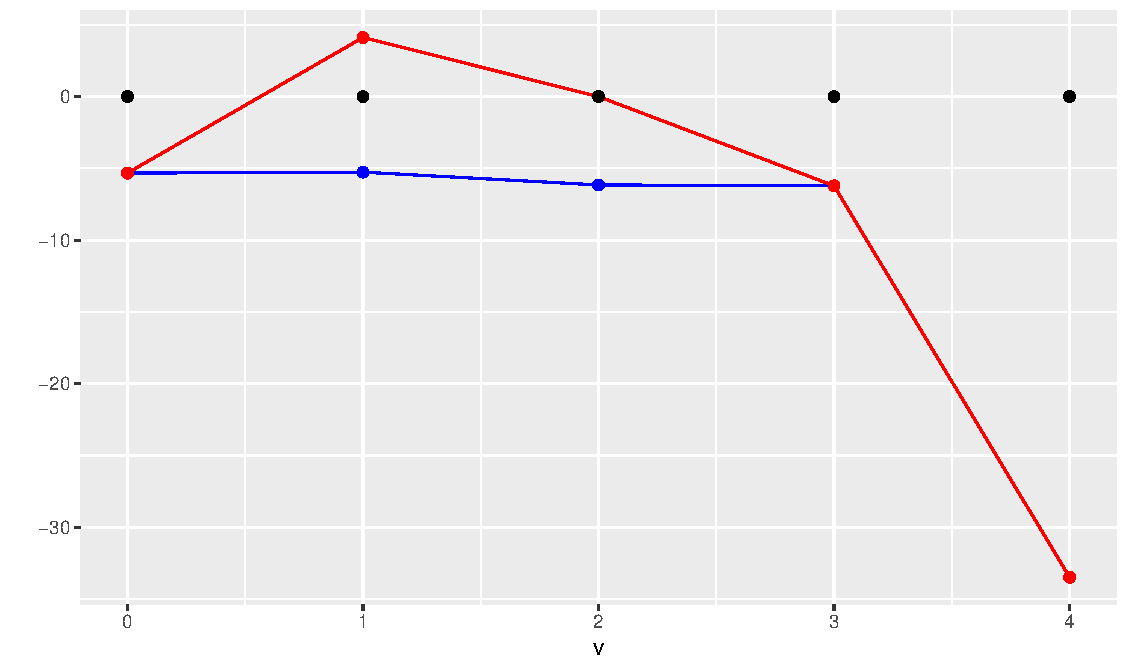
\includegraphics[scale=0.6]{plot1.pdf}
\caption{Upper (red) and lower (blue) critical values and observed values (zero, black) by additional superset size $v$. The bounds for $v=4$ have not been computed in the analysis.}
%\label{fig:bounds}
\end{figure}


\begin{table}[h!]
\centering
\begin{tabular}{cccccc}
\toprule
$v$ & 0 & 1 & 2 & 3 & 4\\
\midrule
$U_v$ & -5.26 & 4.19 & 1.38 & -5.24 & (-32.53)\\
$L_v$ & -5.26 & -5.06 & -4.93 & -5.24 & (-32.53)\\
\midrule
rejection & T & ? & ? & T & T\\
\bottomrule
\end{tabular}
\end{table}


\newpage

\vspace{5mm}
\paragraph{Branch and Bound when removing the highest statistic.}
The last index in $\mathbf{D}$, $i=1$, determines the branching rule. We explore first the subspace where the index is removed.


\begin{table}[h!]
\centering
\begin{tabular}{c|ccccccc}
 & \multicolumn{3}{c}{remove} & & \multicolumn{3}{c}{keep}\\
 & \multicolumn{3}{c}{$S\subseteq V\subseteq F\setminus\{1\}$} & & \multicolumn{3}{c}{$S\cup\{1\}\subseteq V\subseteq F$}\\
\cline{2-4} \cline{6-8}
2 & $\{2,3,4\}$ & $\{2,3,5\}$ & $\{3,4,5\}$ & & $\{1,2,3\}$ & $\{1,3,4\}$ & $\{1,3,5\}$ \\
1 & $\{2,3\}$ & $\{3,4\}$ & $\{3,5\}$ & & & $\{1,3\}$ &  \\
\end{tabular}
\end{table}

%In the "remove" branch, the lower bound remains the same, as the sum of the last $v$ columns of $M$ is not affected by the removal of the first column. However, the upper bound changes in both branches, as the elements corresponding to $i=1$ (in $I$) are removed.





\end{document}